
%%%%%%%%%%%%%%%%%%%%%%%%%%%%%%%%%%%%%%%%%%%%%%%%%%%%%%%%%%%%%%%%%%%%%%%%%%%%%%%%
%2345678901234567890123456789012345678901234567890123456789012345678901234567890
%        1         2         3         4         5         6         7         8

\documentclass[a4paper, 10 pt, journal,compsoc]{IEEEtran}  % Comment this line out
                                                         

\IEEEoverridecommandlockouts                              % This command is only
                                                          % needed if you want to
                                                          % use the \thanks command
\overrideIEEEmargins
% See the \addtolength command later in the file to balance the column lengths
% on the last page of the document



% The following packages can be found on http:\\www.ctan.org
\usepackage{graphicx} % for pdf, bitmapped graphics files
\usepackage{subfig}
\graphicspath{{figures/}}
\usepackage{amsmath} % assumes amsmath package installed
\usepackage{amssymb}  % assumes amsmath package installed
\usepackage{color}
%\usepackage[ruled,linesnumbered]{algorithm2e}
%\usepackage{arydshln}
\usepackage{bm} %bold math
\usepackage{kbordermatrix}

% Environment, operator and command definitions
\newtheorem{problem}{Problem}
\newtheorem{example}{Example}
\newtheorem{lemma}{Lemma}
\newtheorem{theorem}{Theorem}

\DeclareMathOperator{\f}{f}
\DeclareMathOperator{\F}{F}
\DeclareMathOperator{\sgn}{sgn}
\DeclareMathOperator{\xor}{xor}

\newcommand{\Pm}{\ensuremath{\mathcal{P}_m}}
\newcommand{\Pn}{\ensuremath{\mathcal{P}_n}}
\newcommand{\absPn}{\ensuremath{\left|\Pn\right|}}
\newcommand{\x}{\ensuremath{\mathbf{x}}}
\newcommand{\Ol}{\ensuremath{\mathbf{O}(l)}}
\newcommand{\Oll}{\ensuremath{\mathbf{O}(l+1)}}
\newcommand{\Op}{\ensuremath{\mathbf{O}_p}}
\def\marhes{{\sc Marhes}}

%% missing parts, action items
\newcommand{\todo}[1]{\par\noindent{\raggedright\textsc{\color{red}#1}%
    \par\marginpar{{\Large\color{red}$\star$}}}}

\title{\LARGE \bf
$@$LEG
}


\author{\IEEEauthorblockN{Alan Mutka\\}
\IEEEauthorblockA{Faculty of Electrical Engineering and Computing\\
University of Zagreb\\
Unska 3\\
10000 Zagreb, Croatia}
}
\begin{document}

\IEEEcompsoctitleabstractindextext{%
\begin{abstract}

\end{abstract}

\begin{IEEEkeywords}
Hopping robot
\end{IEEEkeywords}}

\maketitle
\thispagestyle{empty}
\pagestyle{empty}

\graphicspath{{./Slike/}}

%%%%%%%%%%%%%%%%%%%%%%%%%%%%%%%%%
\section{INTRODUCTION}



Bla bla


\section{Mass-Spring-Damper Model}

 \begin{figure}[!hb]
      \centering
      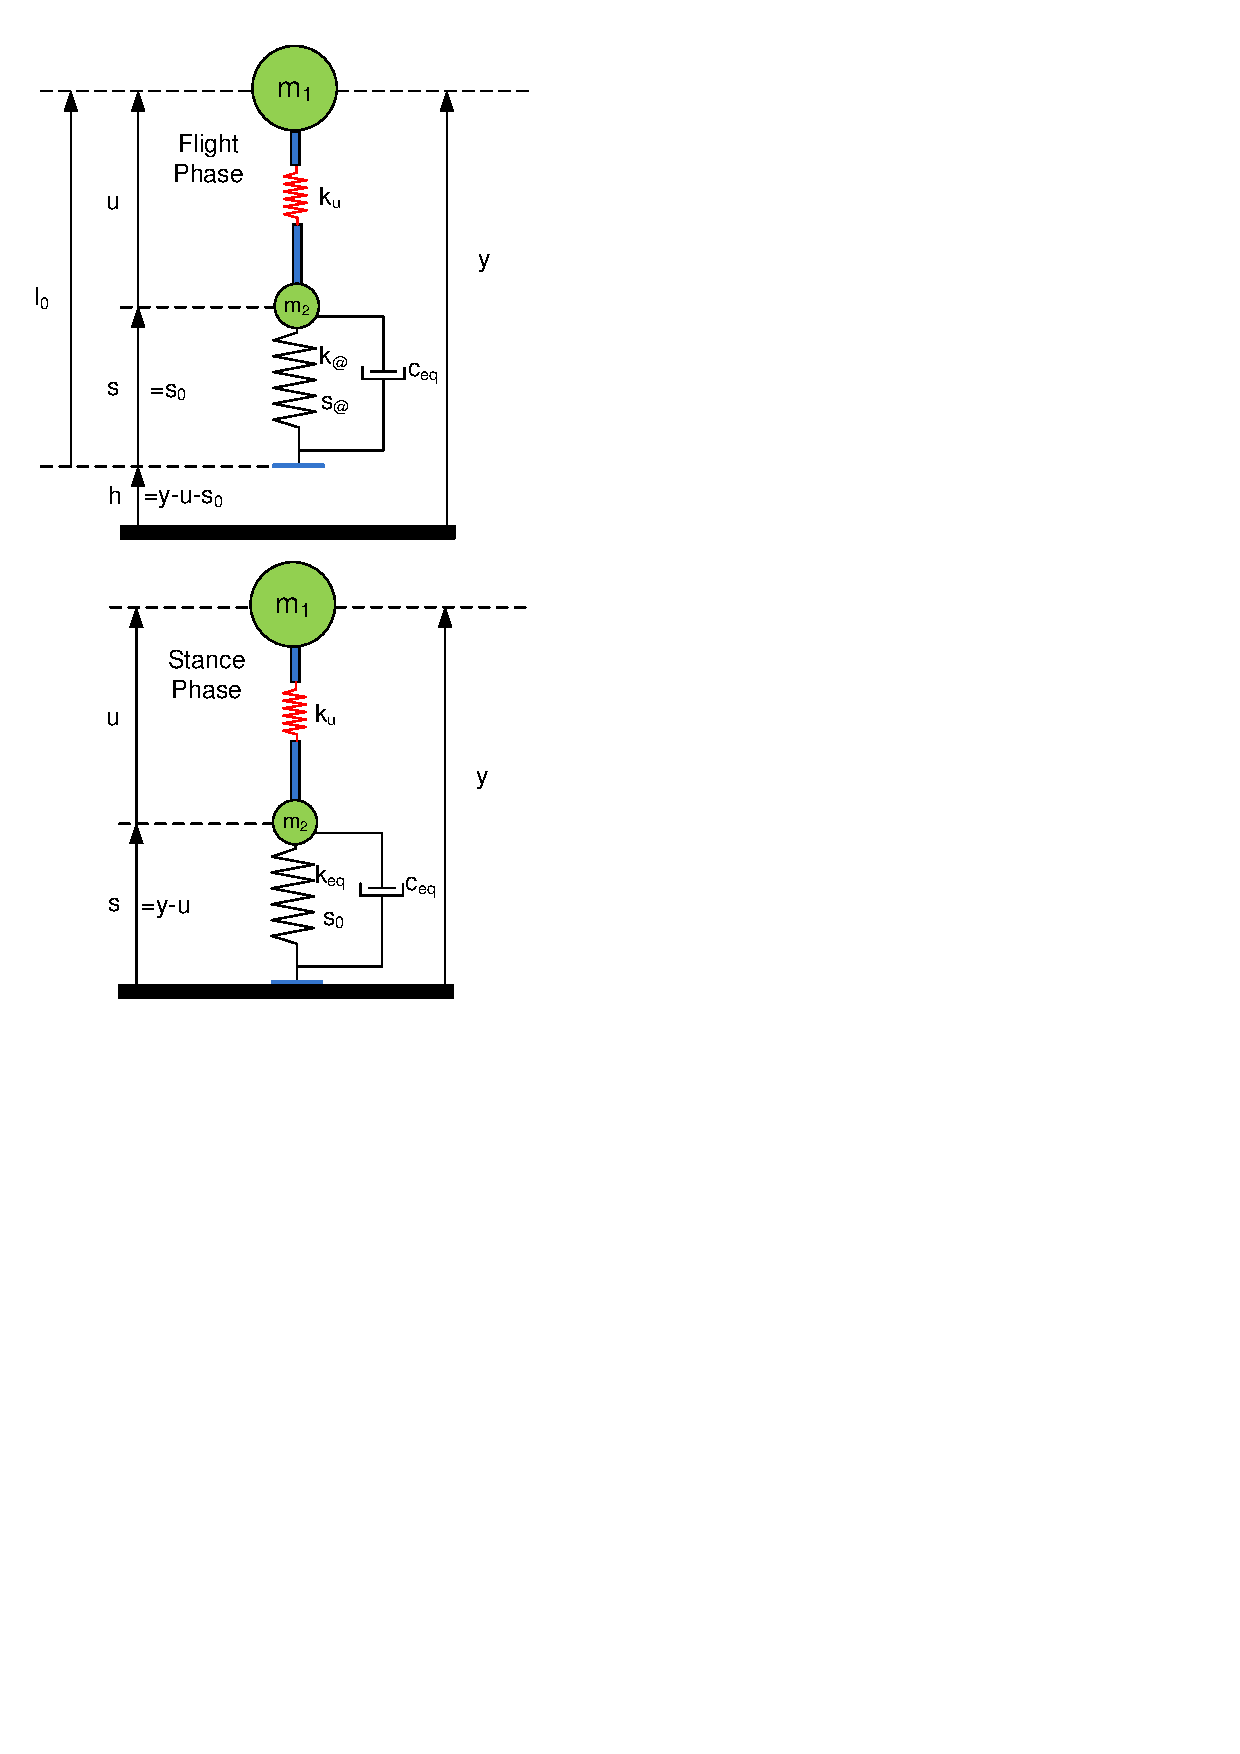
\includegraphics[scale=0.8]{MassSpringDamplerActuator.pdf}
      \caption{MassSpringDamperActuation,flight-stance phase}
      \label{MSDA}
  \end{figure}
 
Introduction to Lagrange Euler  modeling approach.Virtual work. 

The Lagrangian function:
\begin{equation}\label{Lagrangian}
L\left ( q_i,\dot{q_i} \right )=T(q_i,\dot{q_i})-V(y)
\end{equation}
The Lagrangian equation:
\begin{equation}\label{Lagrangian_eq}
\frac{d}{dt}\frac{\partial }{\partial \dot{q_i}}L(q_i,\dot{q_i})-\frac{\partial }{\partial q_i}L(q_i,\dot{q_i})=Q_i
\end{equation}


$Q_i$ - generalized nonconservative force derived by using virtual work principle

Virual work principle assumes infinitesimal virtual displacement on the system which results the virtual work done on the system. 

\begin{equation}\label{virtual_work}
\delta W_j = Q_j\cdot \delta q_j
\end{equation}
  
\subsection{Flight Phase}

The potential energy of $@$LEG (Fig.\ref{MSDA}) is defined as:

\begin{equation}\label{Efpot}
V_{flight}=m_1\cdot g\cdot y+m_2\cdot g(y-u)+\frac{1}{2}k_{u}(u_0-u)^{2}
\end{equation}

where $u_0$ is motor reference position.

The kinetic energy of $@$LEG (Fig.\ref{MSDA}) is defined as:

\begin{equation}\label{Efkin}
T_{flight}=\frac{1}{2}m_1\cdot \dot{y}^{2}+\frac{1}{2}m_2(\dot{y}-\dot{u})^{2}
\end{equation}

The Lagrangian function:

\begin{equation}\label{Lflight}
\begin{split}
L=T_{flight}-V_{flight}=\frac{1}{2}m_1\cdot \dot{y}^{2}+\frac{1}{2}m_2(\dot{y}-\dot{u})^{2} \\
 - m_1\cdot g\cdot y-m_2\cdot g(y-u)-\frac{1}{2}k_{u}(u_0-u)^{2}
\end{split}
\end{equation}

The $@$LEG contains one generalized forces, the spring damping force $Q_c$. Because there is no mass $m_3$ at the end of the leg($s=s_0$), the flight phase does not sense any virtual work.

Two cases of virtual displacement are observed separately.

CASE 1:Suppose there is virtual displacement $\delta y\neq 0$ while $\delta u=0$(by using the (\ref{Lagrangian_eq}) follows):


\begin{equation}\label{flight_fin_1}
(m_1+m_2)\ddot{y}-m_2\ddot{u}+(m_1+m_2)g=0
\end{equation}

CASE 2:Suppose there is virtual displacement $\delta u\neq 0$ while $\delta y=0$(by using the (\ref{Lagrangian_eq}) follows):

\begin{equation}\label{flight_fin_2}
m_2(\ddot{u}-\ddot{y})-m_2g-k_u(u_0-u)=0
\end{equation}

\subsection{Stance Phase}
  
The potential energy of @LEG (Fig.1) is defined as:

\begin{equation}\label{Espot}
V_{stance}=m_1\cdot g\cdot y+m_2\cdot g(y-u)+\frac{1}{2}k_{eq}(s_0-y+u)^{2}+\frac{1}{2}k_{u}(u_0-u)^{2}
\end{equation}

The kinetic energy of $@$LEG (Fig.\ref{MSDA}) is defined as:

\begin{equation}\label{Eskin}
T_{stance}=\frac{1}{2}m_1\cdot \dot{y}^{2}+\frac{1}{2}m_2(\dot{y}-\dot{u})^{2}
\end{equation}

The Lagrangian function:

\begin{equation}\label{Lstance}
\begin{split}
L=T_{stance}-V_{stance}=\frac{1}{2}m_1\cdot \dot{y}^{2}+\frac{1}{2}m_2(\dot{y}-\dot{u})^{2} \\
 - m_1\cdot g\cdot y-m_2\cdot g(y-u)-\frac{1}{2}k_{eq}(s_0-y+u)^{2}
 \\
 -\frac{1}{2}k_{u}(u_0-u)^{2}
\end{split}
\end{equation}
 
Again two virtual displacement are observed separately, $\delta y$ and $\delta u$. Suppose there is virtual displacement $\delta y\neq 0$ while $\delta u=0$.

\begin{equation}\label{virtual_work_stance_1}
\begin{split}
W_{yS} = Q_{yS}\cdot \delta y=-c(\dot{y}-\dot{u}) \delta s \\
s=y-u \Rightarrow  \dot{s}=\dot{y}-\dot{u} \\
\delta s=\delta y, \delta u=0
\end{split}
\end{equation}


Finally:
\begin{equation}\label{virtual_work_stance_3}
Q_{yS} = -c \cdot (\dot{y}-\dot{u})
\end{equation}

Virtual displacement $\delta u\neq 0$ while $\delta y=0$ provides:

\begin{equation}\label{virtual_work_stance_4}
\begin{split}
W_{uS} = Q_{uS}\cdot \delta u=c(\dot{y}-\dot{u}) \delta s \\
s=y-u \Rightarrow  \dot{s}=\dot{y}-\dot{u} \\
\delta s=-\delta u, \delta y=0
\end{split}\end{equation}

Finally:
\begin{equation}\label{virtual_work_stance_5}
Q_{uS} = c \cdot (\dot{y}-\dot{u})
\end{equation}
  

By using the lagrangian Equation (\ref{Lagrangian_eq}) and Equations (\ref{virtual_work_stance_3}) and (\ref{virtual_work_stance_5}) follows:

\begin{equation}\label{stance_fin_1}
(m_1+m_2)\ddot{y}-m_2\ddot{u}+(m_1+m_2)g-k_{eq}(s_0-y+u)=-c(\dot{y}-\dot{u})
\end{equation}

\begin{equation}\label{stance_fin_2}
m_2\ddot{u}-m_2\ddot{y}-m_2g+k_{eq}(s_0-y+u)-k_u(u_0-u)=c(\dot{y}-\dot{u})
\end{equation}
  

 \newpage
  
  
  
  
  


The potential energy of the mass \textit{m} is defined as:

\begin{equation}\label{Epot}
E_{pot}= mg\cdot y(t) + \frac{k\cdot (y(t)-u(t)-l_0)^{2}}{2}
\end{equation}

The kinetic energy of the mass \textit{m} is defined as:

\begin{equation}\label{Epot}
E_{kin}= \frac{m\cdot \dot{y}^{2}}{2}
\end{equation}


By using the Lagrangian function, the equation of motion can be obtained as:

where $F_c$ is damping force defined as:

\begin{equation}\label{DampingForce}
F_c = -c\cdot \left [\dot{y}(t)-\dot{u}(t))  \right ]
\end{equation}



When the leg is in contact with the ground, the final equation of motion is:
\begin{equation}\label{eq1}
m\ddot{y}+c[\dot{y}(t)-\dot{u}(t)]+k[y(t)-u(t)-l_0] = -m g
\end{equation}


The general solution for $y(t)$ and is:

\begin{equation}\label{eq2}
y(t) = e^{\left (-\frac{c}{2m}-iw_d  \right )t}C_1+ e^{\left (-\frac{c}{2m}+iw_d  \right )t}C_2-\frac{gm}{k}
\end{equation}

%\begin{equation}\label{eq2a}
%\dot{y}(t) = (-\frac{c}{2m}-iw_d)e^{\left %(-\frac{c}{2m}-iw_d  \right )t}C_1+ %(-\frac{c}{2m}+iw_d  )e^{\left (-\frac{c}{2%m}+iw_d  \right )t}C_2
%\end{equation}

where $C_1$ and $C_2$ are constants depending on initial conditions and damped natural frequency $w_d$ is defined as:
\begin{equation}\label{eq3}
w_d = \frac{1}{2m} \sqrt{4km-c^{2}}
\end{equation}

When the leg is in contact with the ground the initial conditions are:

\begin{equation}\label{eq4}
\begin{matrix}
y(t) = 0 
\\ 
\dot{y}(t)=-v_0
\end{matrix}\end{equation}

where $v_0$ is the velocity of the ball just prior to contact with the ground. Follows the constant values:

\begin{equation}\label{eq5}
\begin{matrix}
C_1 = \frac{gmw_d}{2kw_d}+i\frac{cg-2kv_0}{4kw_d}
\\ 
C_2 = \frac{gmw_d}{2kw_d}-i\frac{cg-2kv_0}{4kw_d}
\end{matrix}\end{equation}

And the final solution:

\begin{equation}\label{FinalSolution}
y(t)=\left [ \frac{cg-2kv_0}{2kw_d} sin(w_dt)+\frac{mg}{k}cos(w_dt)\right]e^{-\frac{c}{2 m}t} -\frac{mg}{k}
\end{equation}

\subsection{Calculation of total jumping period }
 
The total jumping period consist of time when the leg is in contact with the ground $Tc$  and flight time $Tf$.

The contact time $Tc$ can be obtained from \ref{FinalSolution} by finding the first solution of the equation $y(0)=0$. In order to solve it analytically, the equation \ref{FinalSolution} is rearranged as:


\begin{equation}\label{aprox1}
\begin{split}
y(t)& =-\frac{v0}{w_d}e^{-\frac{c}{2 m}t}\cdot sin(w_dt)\\
& +\frac{mg}{k}\cdot \left [e^{-\frac{c}{2 m}t}(cos(w_dt)+\frac{c}{2mw_d}sin(w_dt)-1  \right ]\\
\end{split}
\end{equation}

Assuming $\frac{mg}{k}<<1$m, which is acceptable for our spring model(see section II), the equation \ref{aprox1} is approximated as:

\begin{equation}\label{aprox2}
y(t) = -\frac{v0}{w_d}e^{-\frac{c}{2 m}t}\cdot sin(w_dt)
\end{equation}

and the minimum non zero solution which represents the contact time $Tc$ is:
\begin{equation}\label{aprox3}
Tc = \frac{\pi}{w_d}
\end{equation}

The flight time $Tf$ is defined as:

\begin{equation}\label{tf}
Tf = \frac{2v_1}{g}
\end{equation}

where

\begin{equation}\label{v1}
v_1 = \dot{y}(Tc)=v_0e^{-\frac{c\pi }{2mw_d}}
\end{equation}


\subsection{Energy loss}

The loss of energy coused by damping factor $c$ can be obtained from difference of kinetic energy $v_0$ and $v_1$:

\begin{equation}\label{dEKIN}
\Delta EKIN = EKINv_1-EKINv_0 = \frac{mv_0^2}{2}\left (e^{\frac{-c\pi}{mw_d}}-1  \right )
\end{equation}

The same energy loss can be obtained with:

\begin{equation}\label{dEcloss}
E_{Closs} = \int Fd\cdot dy=\int (c\cdot \frac{dy}{dt})\frac{dy}{dt}dt =\int_{0}^{T_c} c\dot{y}^{2} dy
\end{equation}

\begin{equation}\label{dEcloss2}
E_{Closs} = \frac{v_0^2\left ( 4m^2+\frac{e^{\frac{-cT_c}{m}\left ( -c^{2}-4m^{2}w_d^{2}+c^{2}Cos[2T_cw_d]+2cmw_dSin[2T_cw_d]] \right )}}{w_d^{2}} \right )}{8m}
\end{equation}







\section{Conclusion}






%%%%%%%%%%%%%%%%%%%%%%%%%%%%%%%%%%%%%%%%%%%%%%%%%%%%%%%%%%%%%%%%%%%%%%%%%%%%%%%%






\begin{thebibliography}{99}

\bibitem{c1} 
L. Righetti and A.J. Ijspeert,Design Methodologies for Central Pattern Generators: An Application to Crawling Humanoids, �in Proc. Robotics: Science and Systems, 2006. 

\bibitem{c2} Chen et al., Locomotion control of quadruped robots based on CPG-inspired workspace trajectory generation, ICRA 2011, pp. 1250-1255, 2011.

\bibitem{c3} Wang et al., Kinematics Analysis and Motion Simulation of a Quadruped Walking
Robot with Parallel Leg Mechanism, The Open Mechanical Engineering Journal, vol. 4, pp. 77-85, 2010.



\end{thebibliography}


\end{document}